% Drawing 154/08-9 -- folder 154, batch 08, archive page 153 (PDF page 154).
% Transcription: en haut, au crayon, deux dessins : un fuseau dont le sommet de droite est traversé de droites marquées $\Delta_1$, $\Delta_\nu$, $\Delta_3$ ; un chapelet de deux fuseaux sur une droite, deux flèches brunes au sommet commun et au sommet de droite
% Kind: pencil spindle with lines Delta_1, Delta_nu, Delta_3 at its right vertex; string of two spindles with brown arrows. Method 2 (schematic redraw from the facsimile). Status: ok.
% Notes: At the top, in pencil, two drawings: a spindle whose right vertex is crossed by lines marked Delta_1, Delta_nu, Delta_3 (labels read « Delta_1 », « nu », « Delta_3 » at this size); a string of two spindles on a line, two brown arrows at the common vertex and at the right vertex. The sketches lower on the page are not covered by this mark. Read from the page view.
% Coordinates: 1 unit = 1 mm = 1/100 of the crop width (bbox in page fractions: [0.171, 0.089, 0.937, 0.204]).
% Redrawn by Claude (claude-opus-5-5), issue #73, 2026-11-07; not checked by a human; not compiled (no TeX in the session).
% Revised 2026-11-07 after Michel's check: correct, except the concurrent point of the left figure; the line nu and Delta_1 now pass exactly through the right vertex of the spindle. Labels enlarged.
% Rights: reproduces part of the work -- behind RENDER_TRANSCRIPTS, never published by itself.
\documentclass[tikz,border=3pt]{standalone}
\usepackage{amsmath,amssymb}
\usetikzlibrary{patterns,arrows.meta}
\tikzset{Or/.style={orange!90!black}, Ye/.style={yellow!80!orange}, Lg/.style={green!60!black!70}, Dg/.style={green!45!black}, Br/.style={brown!80!black}, Rd/.style={red!85!black}, Bl/.style={blue!70!black}, Gy/.style={black!40}, pencil/.style={black!45}, struck/.style={black!35}, mark/.style={circle,draw,inner sep=1.3pt}, pt/.style={circle,fill,inner sep=0.9pt}, opt/.style={circle,draw,fill=white,inner sep=1.1pt}}
\begin{document}
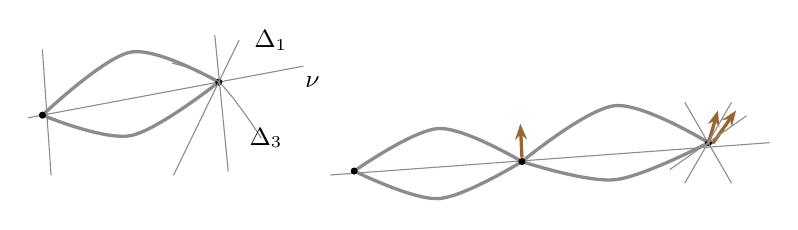
\begin{tikzpicture}[x=1mm,y=1mm,line cap=round,line join=round,font=\scriptsize]
\draw[pencil,very thick] plot[smooth, tension=0.55] coordinates {(3,-10.7) (14.2,-2.7) (25.4,-6.5)};
\draw[pencil,very thick] plot[smooth, tension=0.55] coordinates {(3,-10.7) (14.2,-13.3) (25.4,-6.5)};
\draw[pencil] (1.2,-11.04) -- (36.1,-4.49);
\node[pt] at (3,-10.7) {};
\node[pt] at (25.4,-6.5) {};
\draw[pencil] (3,-2.4) -- (4.1,-18.3);
\draw[pencil] (19.67,-18.3) -- (27.97,-1.2);
\draw[pencil] (24.9,-0.6) -- (26.6,-17.8);
\draw[pencil] plot[smooth, tension=0.55] coordinates {(19.5,-4.1) (25.4,-6.5) (30.8,-13.6)};
\node[inner sep=1pt] at (32,-1.2) {\small $\Delta_1$};
\node[inner sep=1pt] at (37.3,-6.5) {\small $\nu$};
\node[inner sep=1pt] at (31.4,-13.6) {\small $\Delta_3$};
\draw[pencil] (39.6,-18.3) -- (95.3,-14.2);
\draw[pencil,very thick] plot[smooth, tension=0.55] coordinates {(42.6,-17.8) (53.3,-12.4) (63.9,-16.6)};
\draw[pencil,very thick] plot[smooth, tension=0.55] coordinates {(42.6,-17.8) (53.3,-21.3) (63.9,-16.6)};
\draw[pencil,very thick] plot[smooth, tension=0.55] coordinates {(63.9,-16.6) (75.7,-9.5) (87.6,-14.2)};
\draw[pencil,very thick] plot[smooth, tension=0.55] coordinates {(63.9,-16.6) (75.7,-18.9) (87.6,-14.2)};
\node[pt] at (42.6,-17.8) {};
\node[pt] at (63.9,-16.6) {};
\node[pt] at (87.6,-14.2) {};
\draw[Br,very thick,-{Stealth[length=2mm]}] (63.9,-16) -- (63.7,-11.8);
\draw[Br,very thick,-{Stealth[length=2mm]}] (87.6,-14.2) -- (88.8,-10.1);
\draw[Br,very thick,-{Stealth[length=2mm]}] (88.2,-14.2) -- (91.1,-10.1);
\draw[pencil] (82.7,-17.6) -- (92.4,-10.8);
\draw[pencil] (84.6,-19.3) -- (90.5,-9.1);
\draw[pencil] (90.5,-19.3) -- (84.6,-9.1);
\end{tikzpicture}
\end{document}
